\documentclass{standalone}
\usepackage{tikz, pgfplots, amssymb, amsmath, amsfonts}
\pgfplotsset{compat=1.18}
\usetikzlibrary {arrows.meta}
\newcommand{\vect}[1]{\boldsymbol{\mathbf{#1}}}
\begin{document}
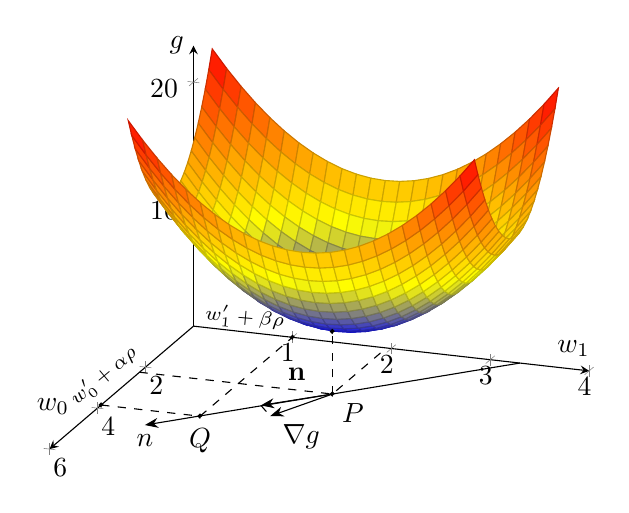
\begin{tikzpicture}
    \begin{axis}[
        grid=major, axis lines=center,
        view={110}{25},
        xmin=0,xmax=+6,
        ymin=0,ymax=+4,
        zmin=0, zmax=23,
        xlabel=$w_0$,
        ylabel=$w_1$,
        zlabel={$g$},
        zlabel style={at={(ticklabel* cs:1)},anchor=east},
        ]
    \addplot3[surf, domain=0.25:3.75, domain y=0.25:3.75] 
        {3*(x-2)^2+3*(y-2)^2+5};
    \draw[dashed](2.25,1.95,0)coordinate(a)node[below right]{$P$}node[draw, circle, fill=black, inner sep=0.5pt]{}--(2.25,1.95,5.1275)node[draw, circle, fill=black, inner sep=0.5pt]{};
    \draw[dashed]coordinate(b)at(3.5,1.625,0);
    \draw[dashed](2.25,0,0)--(a)--(0,1.95,0);
    \draw[-Stealth](a)--(b)node[midway, label=below:{$\nabla g$}]{};
    \draw[dashed](3.85,0,0)node[draw,fill=black, circle,inner sep=0.5pt]{}coordinate(a)--(3.85,1,0)node[draw, circle, fill=black,inner sep=0.5pt,label=below:{$Q$}]{}--(0,1,0)coordinate(b)node[draw,fill=black, circle,inner sep=0.5pt]{};
    \draw(a)node[above,rotate=40,anchor=225]{\scriptsize$w_0'+\alpha\rho$};
    \draw(b)node[above,rotate=-5,anchor=343]{\scriptsize$w_1'+\beta\rho$};
    \draw[dashed](3.086,1.43)--(3.5,1.625);
    \draw[-Stealth](2.25,1.95)--(3.086,1.43)node[midway, label={$\vect{n}$}]{};
    \draw[Stealth-](4.5,0.6)node[below]{$n$}--(0,3.3);
    \end{axis}
\end{tikzpicture}
\end{document}